
\section{RESULTS}
\label{sec:results}

Of course, this simulation has an extensive list of parameters and moving parts, which means that, by necessity, 
there are nearly endless possibilities for analysis. More than twenty variables were left to be varied at the command line, 
each of them able to take on an infinite number of values. To direct our study, we decided to focus on the effects of the 
importance of race (the race weight) on the simulation as well as the potential effects of implementing various policies, 
which included mandated interracial friendships and the construction of forcibly integrated groups.

For the subsequent analyses, we obtained data for each parameter set by running the simulation for ten trials. Information about each student was recorded for every year of the 
simulation, and for each piece of anlaysis, we extracted the variable of interest by transforming this output into two vectors: one documenting the white students and another documenting the minority students. Each element of the vector corresponded to the parameter of interest. Often, this was the proportion of that individual's friends which were 
minorities, but on occasion we were interested in other variables. To prevent duplicates in the data, since a student who attended the college for four years would be included in the file four 
times, we considered only the data that was obtained during a student's senior year. With regards to friendship proportions, it is important to note 
that having no minority friends when you have some number of friends is potentially much different from having no 
minority friends when you have no friends in general. So, we also omitted the data where a student had zero total friends in the case where vectors represent proportions.
After creating a vector for each trial run, we concatenated the ten vectors. The resultant vectors were around 160,000 in 
length for the white data and around 40,000 in length for the minority data.

For the vector comparisons, we chose to use the Wilcoxon rank test (as opposed to the more common Student's t-test) because our data is decidedly non-normal. Figure 1 illustrates this 
fact by using the proportional data as an example. A histogram of all proportional data for one set of ten trials (both white and minority data included) is most closely modeled by the Beta distribution instead of a normal distribution.
\begin{figure}[h]
  \centering
    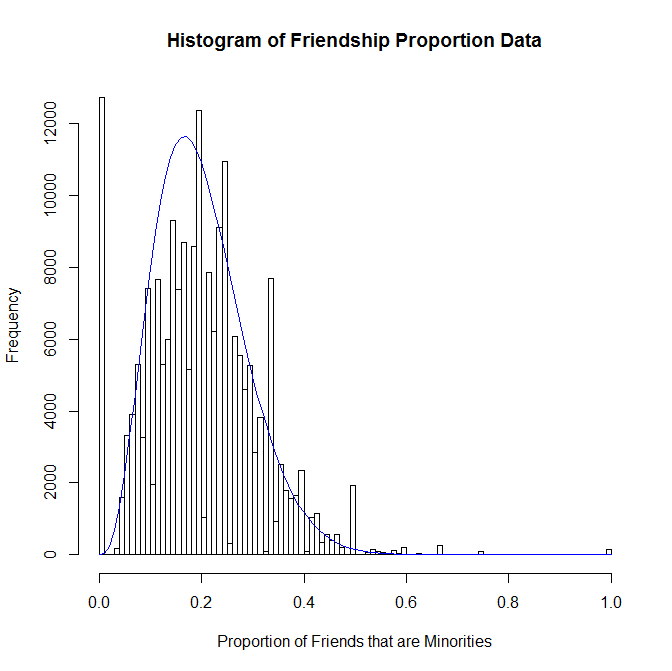
\includegraphics[width=0.5\textwidth]{histogramProportionData.png}
      \caption{A histogram of the proportional data compared to the Beta distribution.}
\end{figure}
We will be using the standard $\alpha=0.05$ rejection value for $p$.

\begin{figure}[h]
  \centering
    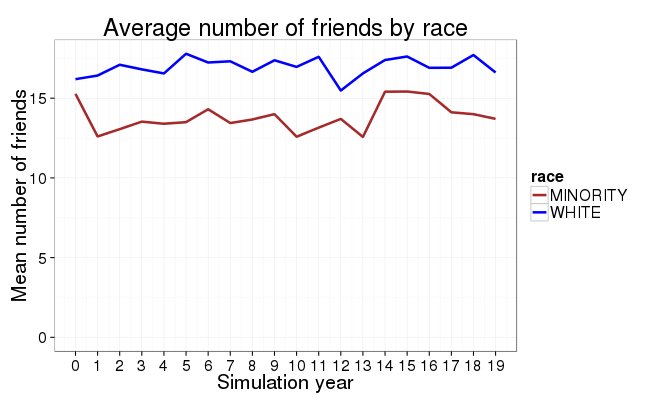
\includegraphics[width=0.5\textwidth]{avgNumberOfFriendsFromCaladan.png}
      \caption{The average number of friends students possessed for one run of the simulation.}
\end{figure}
First, it is important to inspect the data of the average number of friends held by minorities and whites across the years 
in the simulation. An example of such data is shown in Figure 2. Note that for any nonzero race weight, 
minorities had fewer friends on average than whites, regardless of other parameter settings. The following table shows the average 
number of friends held by each of the two races, with the associated $p$-value obtained to determine the difference.
\begin{center}
\begin{tabular}{|c|c|c|c|}
\hline
Race Weight & Average Number of Friends: White & Average Number of Friends: Minority & $p$-value\\
\hline
0 & 15.66 & 15.73 & 0.0784\\
10 & 15.54 & 14.15 & $<2.2\times 10^{-16}$\\
20 & 15.49 & 12.97 & $<2.2\times 10^{-16}$\\
100 & 15.43 & 7.90 & $<2.2\times 10^{-16}$\\
\hline
\end{tabular}
\end{center}~~\\

That is, if race matters even slightly to the students in the simulation, then minorities will form fewer relationships. When race is not a factor in 
forming relationships, the races have an approximately equal average number of friends, as expected. Additionally, the number of friends held by whites 
does not vary for varying race weight, indicating that the level of segregation does not directly impact their ability to form and maintain relationships.

By creating stacked histograms of the racial composition of each group, we observed that the composition of groups at the null 
race weight matched the expected composition, which was based on the population composition, more closely than any of the 
nonzero race weights. As race weight increased, the observed group composition grew farther from that which was expected. In 
fact, at the most extremely high values of race weight, an increasing proportion of the groups consisted only of white 
students, as minorities lose affinity towards many groups, and thus can neither join nor remain in them.

We used boxplots to track and display the frequency of perceived similarity levels whenever two students encountered each 
other. For the null race weight, the interracial encounters experienced the same perceived similarity levels as the 
encounters between two students of the same race. These similarity ratings spread between 0.8 and 1.0. For higher values of 
race weight, the homogeneous race interactions remained at approximately this level. Meanwhile, the perceived similarity of 
heterogeneous race interactions creeped lower. Because of this, homogeneous encounters resulted in friendship slightly more 
often than heterogeneous encounters as race weight was given positive value. As the importance of race increased, the number 
of heterogeneous encounters which resulted in friendship expectedly decreased. However, the number of homogeneous encounters 
which resulted in friendship stayed approximately the same.

After preliminary analyses utilizing various graphs, we proceeded to analyze the data in a more concrete manner. For the following observations, we 
choose to use the proportional friendship data.

%The data generated from race weight being set to 0 was used as our baseline reference 
%for purely integrated data. So, any comparion of data to this baseline reference that was insignificant could be called integrated. The data generated 
%from race weight equalling 100 was considered to be the extremely segregated reference point. Of course, race weight is unbounded, and it would 
%be impossible to find ``the absolute" maximum race weight to case 100\% segregation. We decided that at level 100, race weight is high enough 
%to be deemed extreme segregation. So, any comparison of data to this reference point that was insignificant could be called extremely integrated.

%Some weird results from this so I won't consider it for now

First, we generate a set of vectors for several given weights for race. A second set of vectors was generated using the same parameter sets as the first, but with the 
exception that we have ``turned on" a policy. An inactive policy, one whose parameter was previously zero, was set to have some nonzero parameter. Primarily, 
we investigated the potential effects of creating five intentionally integrated groups at the beginning of each year. We then 
determine if the policy had an effect by performing a Wilcoxon rank test on the sets of vectors - whites when policy is off versus whites when policy is on, and minorities when policy is off 
versus minorities when policy is on - to determine whether or not the policy had a measurable effect on the population.

For the null race weight, the policy does not demonstrate any significant effect on the population. The policy also did not have an effect when race weight was 1, leaving 
the campus still as segregated as it was before the policy was implemented. These results were repeated when race weight was 
set to 10. When the weight of race was increased to 20, the white population did have a significant change after the policy came ``on." The actual difference may 
be unexpected: The policy caused the mean proportion of minority friends held by whites to {\emph decrease}, from 0.1646 to 0.1634. This is evidence that the policy actually caused higher segregation for whites. However, the positive result is that the mean proportion of minority friends held by minorities also decreased, from 0.2215 to 0.2201. This means that, on 
average, minorities were making more friends with whites, improving the integration from their direction. Finally, for the extreme setting of race weight at 100, the policy had a significant effect on the white data, decreasing the mean from 0.0935 to 0.0926. We also briefly investigated the effects of using ten integrated groups instead of five. When race weight equalled 1, we continued to demonstrate the effect that the policy decreases, on average, the proportion of minority friends held by white students. Again, the average proportion of minority friends 
held by minorities also decreased.
%I left out that there was a non-significant effect on the minority data where the mean
%actually went up, so it's almost like the policy made things worse

%If a minority has fewer minority friends, they have more white friends, which means they experience more
%integration. Does that really help them at all? If I'm a minority, am I better off under a policy that causes me
%to have more white friends than I would have been otherwise? Or would it not be as much of an improvement as if I just had
%more friends in general? Or, would I feel more accepted if I could make lots of friends with people of my own race? Is the
%end game to make whites have more minority friends, or to make minorities have more white friends? Which is truly the most
%beneficial in terms of making minorities feel more accepted? Stephen?

%I could see the argument for "minorities having more friends that are white" being beneficial from the viewpoint that
%then they may not feel as threatened by other whites they encounter (may feel more at home/relaxed) as well as that the 
%spread of ideas due to interaction with people who are different is increased.

Finally, we momentarily examined the effects of using a different policy - forced interracial friendships - on the 
populations. We set the number of forced interracial friendships to be 10, a value which is relatively high given the average total number of friendships (see table). At race weight 
set equal to 1, the policy had an effect on both races in the population, again decreasing the mean proportion of minority friends held by both groups. When this was repeated for race 
weight set to 20, the policy appears to have had no effect. It may be that even at a relatively low value for the importance of race, the policy is already not strong enough to overcome 
the perceived barrier.

Clearly, there is a wealth of analysis to be done on this simulation, and we have barely even brushed the surface of the 
possibilities. In future analyses, we hope to collect data on more combinations of the parameters. We seek to determine how 
extreme a policy must be for it to effectively integrate the population for a variety of race weights. Obviously, the null 
weight for race displayed integration regardless of policy status. Other than that, we failed to achieve pure integration 
with any one other policy. It may be that the policies need be more severe, or that we must use the policies in 
conjunction. It also may be that the policies struggle at this proportion of minorities in the population, but would 
excel if the number of minorities was marginally increased. There are an innumerable number of questions to be posed 
surrounding this simulation, and an even wider expanse of data to be collected.
